\documentclass{article}
\usepackage{tikz}
\usetikzlibrary{graphs,graphdrawing}
\usepackage{caption}

\usepackage{multirow}
\usepackage{multicol}
\usepackage[framemethod=tikz]{mdframed}
\usepackage{lipsum}
\usepackage{tkz-graph}
\usegdlibrary{trees}
\usepackage{amsmath, amssymb}
\usepackage{pst-node}
\usepackage{blkarray}
\usepackage{amsmath, amssymb}
\usepackage{pst-node}

\usepackage[margin=2cm]{geometry}

\usepackage[utf8]{inputenc}
\begin{document}
	\section{Esercitazione 6}
	\subsection{Esercizio 1}
	
	Si supponga di volere modellare il comportamento di una semplice lampadina. Si consideri il tempo scandito in
	modo discreto (di secondo in secondo) e che i problemi che possono presentarsi siano i seguenti:
	
	\begin{enumerate}
		\item La lampadina può fulminarsi e smette di funzionare con probabilità 0.05.
		\item La lampadina può risultare troppo calda, per cui ha difficoltà ad accendersi. La probabilità che la lampadina si
		possa surriscaldare troppo vale 0.15 e che in tale situazione abbia probabilità 0.35 di accendersi.
	\end{enumerate}
Si supponga inoltre che il sistema (perfetto) di rilevazione degli errori che si intende utilizzare per verificare il corretto
funzionamento della lampadina indichi l’assenza di errori (good) o la presenza di errori (bad).
Modellare il problema mediante una catena di markov nascosta.

\textit{Per problemi di traduzione il testo è un po' ambiguo ma con "lampadina si
	possa surriscaldare troppo vale 0.15" si intende che la probabilità di diventare o rimanere surriscaldata è sempre 0.15 }

\begin{itemize}
\item	Quali sono gli stati?
\end{itemize}

\[ \Omega = { OK, \; HOT,  \; KO  }\]

\begin{itemize}
		\item Quali sono le possibili osservazioni?
\end{itemize}

\[
	\Sigma = { good, \; bad}
\]

\begin{itemize}
	\item Quali sono le distribuzioni di probabilità di cui abbiamo bisogno?
\end{itemize}

\begin{enumerate}
	\item Distribuzione iniziale di probabilità: \[\pi = (0, 0, 1)^T \] \\
	     Assumiamo che inizialmente la lampadina sia sempre funzionante
	     
	\item Matrice di transizione $A$ 
	\[
	A = 
	\begin{blockarray}{cccccc}
		& OK & HOT & KO \\
		\begin{block}{c(ccccc)}
			OK &	0.8 &  0.15   & 0.05   \\
			HOT &	0.8 &  0.15   & 0.05 \\
			KO &	0   &  0      & 1   \\
		\end{block}
	\end{blockarray}
	\]	
	
	\item Matrice di emissione delle osservazioni.
	
	\begin{mdframed}[hidealllines=true,backgroundcolor=blue!20]
		La matrice di emissioni delle osservazioni mi dice per ogni stato quali osservazioni posso emettere.
	\end{mdframed} 
		\[
	E = 
	\begin{blockarray}{cccccc}
		& Good & Bad \\
		\begin{block}{c(ccccc)}
			OK  &	1    &  0   \\
			HOT &	0.35 &  0.65   \\
			KO  &	0    &  1      \\
		\end{block}
	\end{blockarray}
	\]	

\pagebreak

\begin{itemize}
 \item  Qual è la rappresentazione grafica dell' HMM?
\end{itemize}
	\begin{center}
		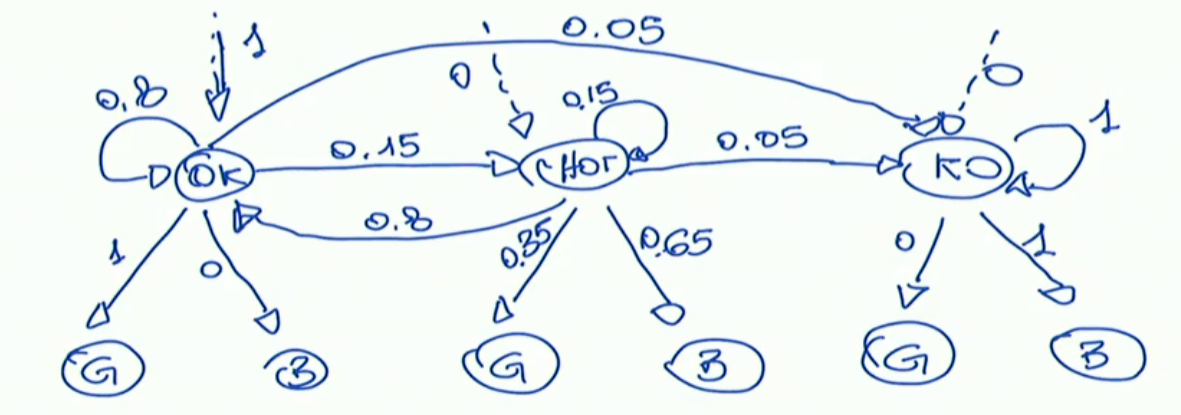
\includegraphics[width=12cm]{./immagini/hmm_es1.png}
	\end{center}
	
\end{enumerate}

\pagebreak
	\subsection{Esercizio 2}
	Dato un HMM caratterizzato da:
	\begin{itemize}
		\item Un insieme di stati $S = \{S_1, ..., S_k\}$
		\item Un insieme di osservazioni  $O = \{O_1, ..., O_m\}$
	\end{itemize}
	
	Quanti parametri sono necessari per definire un HMM?
	
	I parametri necessari sono:
	
	\[
		k + k^2 + km
	\]
	
\begin{itemize}
	\item $k$ rappresenta ciò che prima abbiamo chiamato $\pi$, ovvero il \textbf{vettore delle probabilità iniziali}. \\
	Sarà un vettore $\pi = [1, ..., k]$
	
	\item $k^2$ rappresenta la matrice di transizione fra gli stati, quella che prima abbiamo chiamato $A$.
	
	\item $km$ è una matrice che rappresenta le possibili osservazioni che uno stato può produrre, quella che priam abbiamo chiamato $E$.
\end{itemize}

L'unione di questi parametri ci consente di specificare un HMM

\pagebreak

\subsection{Esercizio 3}

Consideriamo questo HMM:

Vettore delle probabilità iniziali
\[P  = 0.5; 0.5;\]

Matrice di transizione $T$
\[
T = 
\begin{blockarray}{cc}
	\begin{block}{(cc)}
		0.3  &  0.7   \\
		0.4  &  0.6   \\
	\end{block}
\end{blockarray}
\]	

Matrice di emissione delle osservazioni  $O$
\[
O = 
\begin{blockarray}{cc}
	\begin{block}{(cc)}
		0.4  &  0.6   \\
		0.8  &  0.2   \\
	\end{block}
\end{blockarray}
\]	
\end{document}


